\section{メメティックアルゴリズムと CIM の生成条件}\label{sec:ga}

\subsection{タブー探索の不具合と，CIM 初期集団の再評価}

メメティックアルゴリズム（GA）\cite{wu2012}は，交叉で作った子をタブー探索（TS）で磨き，距離と品質で集団を更新する．以前の実験では，G70 で CIM の解だけで作った初期集団の GA が 300 世代の間まったく改善せず，G55 では CIM 初期集団がランダムな初期集団より悪かった．原因を調べたところ，TS の実装が，利得が最大の非タブーの手が複数あるときに常に番号最小の頂点を選んでいた．疎なグラフの局所最適解には利得 0 の手が多数残るので，TS は同じ数頂点を往復し続け，局所最適解から動けなかった．Wu と Hao\cite{wu2012}にならい，同点の手を等確率に選び，摂動の強さを 150 にした．

同点を等確率に選ぶと，全頂点を走査しながら同点のたびに乱数を引くので，TS が遅くなった（40000 反復で G55 で 2.6 倍，G70 で 6.2 倍）．そこで，非タブーの頂点を利得の値ごとの配列（バケット）で管理し，最大利得のバケットから乱数 1 回で選ぶようにした．タブーの頂点はバケットから外してリストで管理し，aspiration はリストだけを調べる．選ぶ規則は全走査と同じであり，毎反復の状態を全走査の結果と照合する検査で食い違いがないことを確かめた．走査版に比べ，40000 反復で G22 で 2.8 倍，G55 で 31 倍，G70 で 87 倍速くなった．

修正後の TS で，以前と同じ seed・同じ初期集団（各問題 16 回，300 世代）の実験をやり直した（図\ref{fig:ga}）．G55 と G70 では結論が逆になった．300 世代後の BKS との差は，G55 で CIM 初期集団 $56.2\pm3.8$ に対しランダム $63.1\pm2.9$，G70 で $72.4\pm3.0$ に対し $92.2\pm3.6$（平均 $\pm$ 標準誤差）であり，CIM 初期集団のほうが良い．以前の「CIM 初期集団は GA の役に立たない」という結果は，TS の不具合によるものだった．G22 ではどちらも BKS との差 0.9 で差がなかった．この比較は同じ世代数での比較であり，CIM の生成時間は含めていない．生成時間を含めた比較は次の小節で行う．

\begin{figure}[t]
\centering
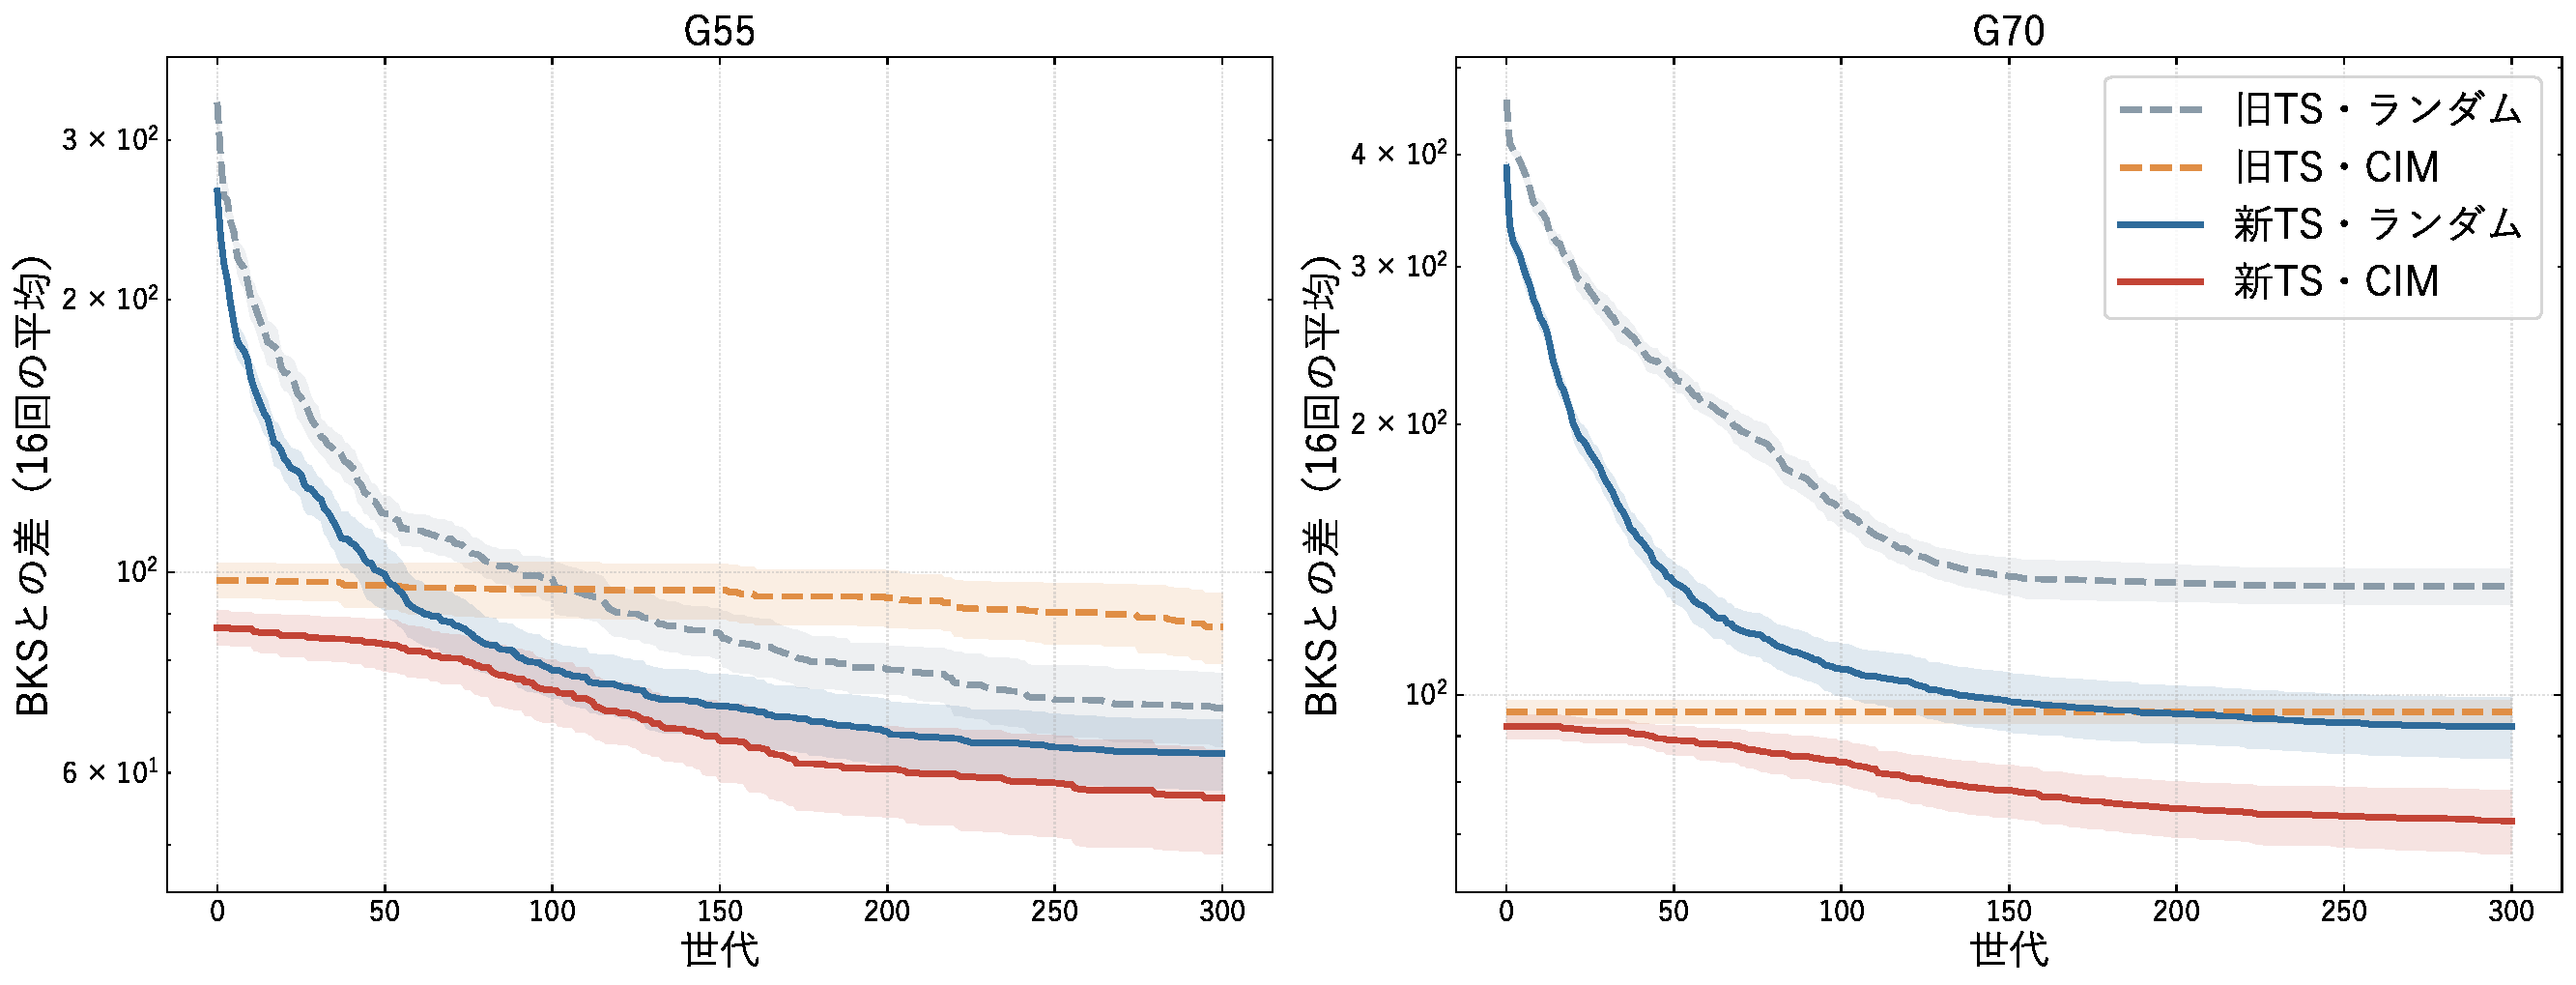
\includegraphics[width=\linewidth]{fig_ga.pdf}
\caption{GA の最良値の推移（BKS との差，16 回の平均と 95\% 区間）．破線は修正前の TS，実線は修正後の TS．同じ seed・同じ初期集団で比べた．}\label{fig:ga}
\end{figure}

\subsection{CIM の生成時間を含めた比較}\label{sec:ga_equal_time}

SA では，CIM の生成時間を後段に回すと，長い予算でランダムな初期解が勝った（\ref{sec:selection} 節）．GA でも同じことが起こるか，また，GA は交叉で解を組み合わせるので，SA では役に立たなかった多様な初期集団が効くかを調べた．条件と判定は実行前に文書に固定した．

問題は G22，G55，G70 で，GA のパラメータと CIM のラウンド数（G22・G70 は 4800，G55 は 9600）は前の小節と同じにした．GA と CIM はともに新しい seed で各問題 16 回実行した．各回で CIM の解を $K=4p$ 個（$p$ は集団サイズ）作り，初期集団を次の 4 通りで作った．\textbf{ランダム}は GA 既定の初期集団である．\textbf{CIM（選別なし）}は $K$ 個のうち seed 順に先頭の $p$ 個を使い，CIM の時間は $p$ 本分だけ課す．\textbf{CIM＋カット値}はカット値の上位 $p$ 個，\textbf{CIM＋カット値＋ハミング距離}はカット値の上位 $2p$ 個から互いに離れた $p$ 個を貪欲に選び，どちらも CIM の時間を $K$ 本分課す．どの条件も，初期集団に TS をかけてから世代を進める．

時間は，ほかの計算との重なりの影響を受けにくい 1 スレッドの CPU 時間で数えた．CIM 1 本の時間は GA の 1 世代の 32 倍（G22），124 倍（G55），147 倍（G70）だった．評価時刻は「CIM＋カット値が CIM の時間を払って 300 世代進む時刻」（40〜54 秒）とし，各回のその時刻までの最良値を比べた．CIM の時間の倍率 $c$ を 1（主条件）と，物理的な CIM で生成が速い場合を想定した 0.1，0 で変えた．判定は 2 つで，問題ごとに片側検定を行い，3 問題で Holm の補正をかけた．V4a：CIM（選別なし）がランダムより良い（Mann--Whitney の U 検定）．V4b：CIM＋カット値＋ハミング距離が CIM＋カット値より良い（同じ CIM の候補と GA の seed で対応があるので Wilcoxon の符号順位検定）．

\begin{table}[t]
\centering
\caption{CIM の生成時間を含めた GA の比較．評価時刻での BKS との差（\%，16 回の平均）．$c$ は CIM の時間に掛けた倍率．}\label{tab:ga_equal_time}
\small
\begin{tabular}{lccccc}
\toprule
問題 & $c$ & ランダム & CIM（選別なし） & CIM＋カット値 & CIM＋カット値＋距離 \\
\midrule
G22 & 1 & 0.014 & 0.006 & 0.007 & 0.007 \\
G55 & 1 & 0.502 & \textbf{0.316} & 0.441 & 0.572 \\
G55 & 0 & 0.502 & 0.312 & \textbf{0.284} & 0.323 \\
G70 & 1 & 0.861 & \textbf{0.609} & 0.684 & 0.880 \\
G70 & 0 & 0.861 & 0.589 & \textbf{0.556} & 0.754 \\
\bottomrule
\end{tabular}
\end{table}

\begin{figure}[t]
\centering
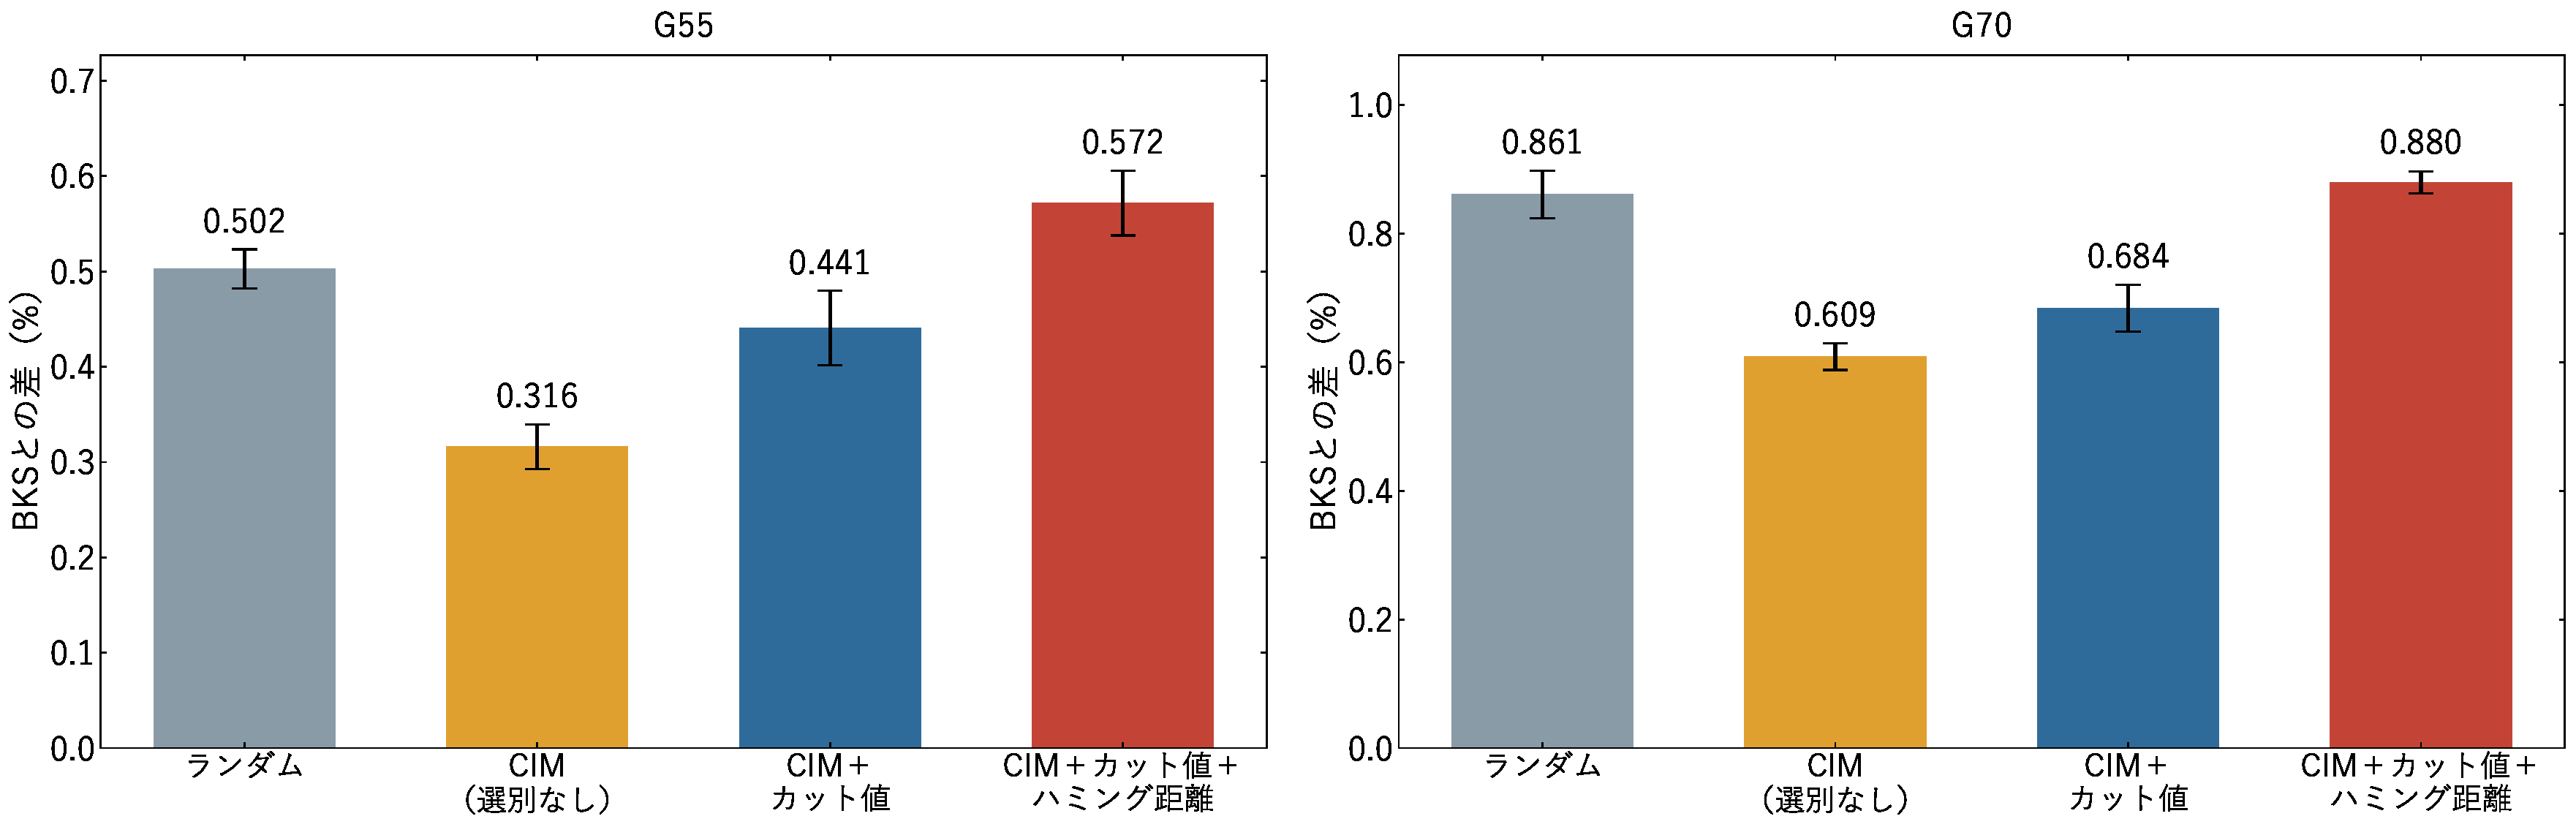
\includegraphics[width=\linewidth]{fig_ga_equal_time.pdf}
\caption{CIM の生成時間を含めた GA の比較（主条件 $c=1$）．評価時刻での BKS との差（16 回の平均と標準誤差）．}\label{fig:ga_equal_time}
\end{figure}

\paragraph{CIM の初期集団は生成時間を含めても良い（V4a 成立）.} G55 と G70 では，CIM（選別なし）がランダムより良かった（表\ref{tab:ga_equal_time}，図\ref{fig:ga_equal_time}．Holm 補正後 $p=2.2\times10^{-5}$，$1.5\times10^{-5}$）．G22 では全条件が BKS から 1〜2 しか離れず，差は出なかった（$p=0.55$）．実行前には，CIM の時間がランダムの数百〜千世代分に当たるので $c=1$ では成り立たないと予想していたが，この予想は外れた．時間と最良値の推移を見ると，ランダムな初期集団の GA は早い段階で伸びが止まる．CIM の初期集団の GA は，CIM の時間（G55 で約 10 秒，G70 で約 13 秒）を払った後，短時間でランダムを追い越し，その後も差が開いた．SA の長い予算と結果が逆になったのは，ランダムな初期解からの SA は本数を増やせば伸びるのに対し，GA の集団は一度停滞すると世代を重ねても抜け出しにくいためと考えられる．

\paragraph{多様な初期集団は役に立たない（V4b 不成立）.} ハミング距離で選んだ集団は，カット値だけで選んだ集団より悪かった（対応のある 16 回で G55 は 3 勝 13 敗，G70 は 1 勝 13 敗，Holm 補正後 $p=1.0$）．$c=0.1$，0 でも同じ向きだった．事後の診断では，各個体の最も近い相手との距離の平均は，G55 でカット値 0.235・選別なし 0.276・ハミング距離 0.320，G70 で 0.217・0.257・0.281 であり，$c=0$ での成績の順（カット値，選別なし，ハミング距離）と一致した．ハミング距離で選んだ集団は，選別なしより平均カット値が高いのに成績が悪い．この GA の交叉は親の共通部分を引き継ぐので，互いに近い個体の組がない集団では引き継げる部分が少ないためと考えられる（事後の解釈）．

\paragraph{時間の見積もりへの感度.} CIM 1 本の時間を 3 回の測定の最小値から中央値に変えた場合と，GA の 1 世代の時間を長い実行の傾きから求めた場合でも，V4a と V4b の判定は変わらなかった．ただし CIM＋カット値は，CIM の時間を中央値にすると評価時刻までに CIM の生成が終わらず，ランダムより悪くなった（G55 で 0.635\% 対 0.502\%）．評価時刻をこの条件に合わせて決めたため，この条件は時間の見積もりに最も敏感である．$c=1$ で CIM＋カット値が選別なしに負けたのも，$K=4p$ 本の CIM の時間を払うためであり，$c=0$ では逆にカット値で選ぶほうが良い．

\subsection{CIM の生成条件と固有ベクトルの系統}

G22 で，候補がどちらの固有ベクトルの系統に入るかを CIM の生成条件で変えられるかを調べた．事前登録の R1 と同じ設定（600 ラウンド，SA 開始温度 2.0・5000 掃引）を基準に，ポンプの立ち上げの速さ（ラウンド数と掛けた最終のポンプ強度は揃えた）と真空雑音の大きさを変え，各条件で新しい seed の候補 256 個に SA を 4 回ずつかけた（表\ref{tab:lineage}）．

\begin{table}[t]
\centering
\caption{G22 で CIM の生成条件を変えたときの候補（各 256 個）．$E>0$ は $u_1$ の系統に入った候補の割合．差は基準との差と 95\% 区間（独立 2 標本の正規近似）．}\label{tab:lineage}
\small
\begin{tabular}{lrcccc}
\toprule
条件 & ラウンド & 平均カット値 & $E>0$ の割合（基準との差） & SA 後の平均（基準との差） & $\rho(E, r)$ \\
\midrule
基準 & 600 & 13238.2 & 0.68 & 13331.0 & 0.44 \\
ポンプ 0.5 倍速 & 1200 & 13245.3 & $+0.06$ [$-0.02$, $0.13$] & $-1.0$ [$-3.5$, $1.5$] & 0.47 \\
ポンプ 2 倍速 & 300 & 13214.1 & $-0.11$ [$-0.20$, $-0.03$] & $-2.2$ [$-4.7$, $0.3$] & 0.45 \\
雑音 0.5 倍 & 600 & 13238.0 & $+0.01$ [$-0.07$, $0.09$] & $-0.1$ [$-2.7$, $2.5$] & 0.48 \\
雑音 2 倍 & 600 & 13237.4 & $-0.00$ [$-0.09$, $0.08$] & $+0.2$ [$-2.4$, $2.7$] & 0.45 \\
雑音 4 倍 & 600 & 13237.8 & $-0.01$ [$-0.09$, $0.07$] & $+0.3$ [$-2.3$, $2.8$] & 0.44 \\
\bottomrule
\end{tabular}
\end{table}

ポンプを速く立ち上げると，$u_1$ の系統に入る候補の割合が下がった（$-0.11$）．線形増幅の段階が短くなり，最大固有値のモードが他のモードに差をつける時間が減るためと考えられる．雑音の大きさは 0.5〜4 倍の範囲で影響しなかった．SA 後の平均は条件によって有意には変わらなかった．一方，$E$ と残差の相関はすべての条件で 0.44〜0.48 であり，G22 で $E$ が効くことは，新しい seed による 6 回の測定でも変わらなかった．系統の割合はポンプの速さで多少動かせるが，その効果は小さく，候補の選別に代わる手段にはならない．
